\RequirePackage[ngerman=ngerman-x-latest]{hyphsubst}

\documentclass[ngerman]{tudscrreprt}

% packages
\usepackage[ngerman]{babel}
\usepackage{booktabs}
\usepackage{bytefield}
\usepackage{caption}
%\usepackage{hyperref}
\newcommand{\url}[1]{{\texttt{#1}}}
\usepackage[utf8]{inputenc}
\usepackage[outputdir=out]{minted}
\usepackage{pmboxdraw}
\captionsetup[table]{position=above}
\usepackage{tabularx}
\usepackage[svgnames,table]{xcolor}
\usepackage[most]{tcolorbox}

% commands
\newtcolorbox[%
  auto counter,
  number within=section,
  list inside=mypyg]{mintedbox}[2][]
  {%
    enhanced,
    breakable,
    enlarge top by=1ex,
    enlarge bottom by=1ex,
    before upper={\parindent15pt\noindent},
    after={\noindent},
    fonttitle=\bfseries,
    title={Listing \thetcbcounter: #2},
    list entry={\protect\numberline{\thetcbcounter}#2},
    #1}

\newminted[mintc]{c}{%
  fontsize=\footnotesize,%
  fontseries=b%
}

\newminted[mintcpp]{cpp}{%
  fontsize=\footnotesize,%
  fontseries=b%
}

\newminted[mintpython]{python}{%
  fontsize=\footnotesize,%
  fontseries=b%
}

\newminted[mintlua]{lua}{%
  fontsize=\footnotesize,%
  fontseries=b%
}

\newminted[minttext]{text}{%
  fontsize=\footnotesize,%
  fontseries=b,%
  escapeinside=~~%
}

\newenvironment{mintlisting}[3][]
 {\def\listingsboxenvironment{#2}
  \VerbatimEnvironment%
  \begin{mintedbox}[#1]{#3}%
    \begin{\listingsboxenvironment}}%
 {\end{\listingsboxenvironment}%
  \end{mintedbox}%
}


\begin{document}

\sloppy

\faculty{Fakultät für Elektrotechnik und Informationstechnik}

\title{Bericht Fachpraktikum}

\author{%
  Timo Nicolai
  \course{Informationssystemtechnik}
  \matriculationnumber{4048209}
}

\authormore{geb. 03.08.1994, Flensburg}

\headingsvskip=-100pt

\maketitle

\confirmation

\tableofcontents

\pagebreak

\chapter{Einleitung}

Vom 11.09.2017 bis zum 20.07.2018 war ich als Werkstudent und später vom
17.06.2019 bis zum 20.10.2019 als Vollzeit-Praktikant bei der Kernkonzept GmbH
angestellt.

Kernkonzept entwickelt das \textit{L4Re Mikrokernel-Betriebssystem}.
Die Entwicklung begann als Forschungsprojekt an der Professor für
Betriebssysteme der TU Dresden. Das Unternehmen wurde von ehemaligen/noch an
der Universität arbeitenden wissenschaftlichen Mitarbeitern gegründet. L4Re
wird zudem weiterhin zu Lehrzwecken an der Universität eingesetzt.

Kapitel~\ref{ch:background} dient der Einführung in die technischen Grundlagen
meiner Arbeit. Abschnitt~\ref{sec:mkos} beschreibt dabei die Grundidee hinter
Mikrokernel-Betriebssystemen und gibt eine Einführung in deren historische
Entwicklung sowie aktuelle Forschungs-Richtungen.  Abschnitte~\ref{sec:l4re}
und \ref{sec:l4re_pi} gehen dann spezifisch auf L4Re ein, es wird insbesondere
ein anschauliches L4Re-Beispielprogramm motiviert und erläutert um das
Verständnis späterer Darstellungen zu erleichtern.  Kapitel~\ref{ch:projects}
beschreibt schließlich die wichtigsten Projekte an denen ich während meiner
Zeit bei Kernkonzept gearbeitet habe und Kapitel~\ref{ch:conclusion} enthält
ein kurzes Fazit.

\vspace{\baselineskip}

\noindent
Hinweis: Für eine Farbkopie dieses Berichtes im PDF-Format, senden Sie eine
Mail an \url{timo.nicolai@mailbox.tu-dresden.de}.

\chapter{Stand der Technik}
\label{ch:background}

\section{Mikrokernel-Betriebssysteme}
\label{sec:mkos}

\subsection{Grundidee}

Mikrokernel sind Betriebssystem-Kernel die lediglich minimale, zur Konstruktion
eines vollständigen Betriebssystems nötige, Funktionalität implementieren, z.B.
Adressräume, Threads und Interprozesskommunikation.

Im Gegensatz zu \textit{monolithischen} Betriebssystemen (wie zum Beispiel
GNU/Linux) werden klassischerweise vom privilegierten Kernel ausgeführte
Grundfunktionen des Systems (z.B. Geräte-Treiber) in User-Space Programme
ausgelagert. Das Grundprinzip hinter modernen Mikrokerneln lautet hierbei
\textit{,,capability, not policy''}: Der Kernel stellt idealerweise lediglich
die zur Nutzung der unterliegenden Hardware nötige minimale Funktionalität
bereit, trifft aber keine strategischen Entscheidungen. Dies wird stattdessen
von einer Reihe von User-Space Programmen übernommen\footnote{Diese Darstellung
ist eine Idealisierung, in der Praxis kann es Sinn ergeben, besonders
Performance-kritische Funktionalität wie z.B.  Scheduling in den Kernel zu
integrieren auch wenn dies das genannte Prinzip verletzt.}

Vorteil ist dabei die verbesserte Stabilität und Sicherheit des Systems.  Ein
kompliziertes System wie Linux mit vielen Millionen Code-Zeilen ist sehr
anfällig für unentdeckte Fehler, welche die Stabilität des Systems gefährden
oder zum Beispiel von einem Angreifer ausgenutzt werden können, um
privilegierte Programme auszuführen.  Die Sicherheit eines Mikrokernels, der in
nur einigen zehntausend Zeilen Code implementiert ist, kann dagegen mit
realistischem Aufwand sehr genau überprüft werden.  Selbst wenn es einem
Angreifer gelingt, ein User-Space Programm zu kompromittieren, bleibt zudem die
Integrität des Kernels unberührt und der potentielle Schaden ist deutlich
geringer da das entsprechende Programm im Bedarfsfall beendet und neu gestartet
werden kann und ohnehin als User-Space Programm nur indirekten Hardware-Zugriff
hat.

Ein weiterer Vorteil ist die Modularität des Systems, User-Space Komponenten
mit identischen Schnittstellen können (sogar zur Laufzeit) untereinander
ausgetauscht werden (vergleichbar mit heute weitverbreiteten
\textit{Microservices}) und das gesamte System lässt sich potentiell einfacher
auf verschiedene physische Maschinen verteilen.

Problematisch ist unter Umständen die Performance des Systems: Mikrokernel
machen viel größeren Gebrauch von Interprozesskommunikation als monolithische
Kernel und diese ist zudem oft synchron. Eine der Herausforderungen bei der
Entwicklung eines Mikrokernel-Systems ist die bestmögliche Bewältigung solcher
Performance-Hürden.

\subsection{Historische Entwicklung}

Die Grundidee hinter Mikrokernel-Betriebssystemen existiert bereits seit den
60er Jahren~\cite{rc4000}. Frühe Mikrokernel, z.B. Mikrokernel Varianten von
\textit{Mach}~\cite{mach} litten vor allem unter Performance Problemen bei der
Interprozesskommunikation.

Großer Fortschritt in diesem Bereich gelang Jochen Liedtke.  Dieser stellte die
These auf, dass schlechte Performance kein inhärentes Problem des
Mikrokernel-Ansatzes, sondern das Resultat suboptimaler Implementierungen war
und entwickelte \textit{L3}~\cite{l3} in dem Interprozesskommunikation über 20
mal schneller war als in Mach. L3 war dabei noch kompakter als vorangegangene
Mikrokernel.

Mit \textit{L4}~\cite{l4} wurde später ein weiterer Mikrokernel entwickelt,
dessen Hauptziel hohe Performance war und der einige weitere in Mach präsente
Probleme umging. Damit wurde die Ära der kompakten und performanten Mikrokernel
der \textit{zweiten Generation} eingeleitet. Es folgten eine Reihe von von L4
basierten Systemen, z.B. \textit{L4Ka::Pistachio}, \textit{L4/MIPS},
\textit{L4/Fiasco} und \textit{OKL4}.

Spätere Mikrokernel der \textit{dritten Generation} legten dann den Fokus auf
\textit{Capabilities}, Virtualisierung und Verifizierbarkeit.

Capabilities sind dabei ein Mechanismus zur Zugriffs-Kontrolle.  Um auf eine
Ressource (z.B. Speicher) zuzugreifen, muss ein Programm eine Capability auf
diese besitzen.  Capabilities können zwischen Programmen ausgetauscht werden,
z.B. kann der Erzeuger einer Ressource Zugriff auf diese an eine Reihe von
Verbraucher weiterleiten. Eine Capability ist sowohl ein Zeiger auf als auch eine
Zugriffs-Berechtigung für einer Ressource.  Zugriffs-Verwaltung lässt sich somit
in den User-Space auslagern. Dieses Prinzip ist deutlich eleganter als
Zugriffs-Verwaltung unter UNIX-ähnlichen Systemen, in denen der Kernel bei
jedem Zugriff auf eine Ressource die Berechtigungen des ausführenden Programmes
überprüfen muss.

Capabilities waren bereits in Mikrokerneln der ersten Generation, z.B. Mach
implementiert aber aus Performance-Gründen kein Teil mehr von Mikrokerneln der
zweiten Generation.  Diese verwendeten alternative Ansätze die sich im
Nachhinein als suboptimal entpuppten. Mikrokernel der dritten Generation
implementieren Capabilities auf effizientere Art und Weise, die es gleichzeitig
erlaubt, die Verfügbarkeit von Ressourcen besser zu verfolgen.

Manche Mikrokernel der dritten Generation werden häufig als Hypervisor (z.B.
für ,,unsichere'' monolithische Systeme wie GNU/Linux) eingesetzt, ein Beispiel
ist \textit{Fiasco.OC}~\cite{fiasco}. Da dabei vor allem (sowohl akademisches
als auch kommerzielles) Interesse an der Sicherheit solcher Systeme besteht,
ist Verifizierbarkeit ein aktueller Trend. Mit \textit{seL4}~\cite{sel4}
existiert so z.B. ein Mikrokernel, dessen Sicherheit (ausgehend von gewissen
Axiomen) mathematisch bewiesen ist.

Neben der L4 Familie existieren heute viele weitere ganz oder teilweise den
Mikrokernel-Ansatz verfolgende Betriebssysteme. Beispiele sind das Andrew S.
Tanenbaum ursprünglich als Lehrsystem entwickelte \textit{Minix}, der von
Linux unabhängige \textit{GNU Hurd} Kernel und Googles \textit{Fuchsia/Zircon}.

\section{L4Re}
\label{sec:l4re}

Kernkonzept entwickelt das \textit{L4Re} Mikrokernel-Betriebssystem.
Die Entwicklung begann als Forschungsprojekt an der Professor für
Betriebssysteme der TU Dresden. Das Unternehmen wurde von ehemaligen/noch an
der Universität arbeitenden wissenschaftlichen Mitarbeitern gegründet. L4Re
wird zudem weiterhin zu Lehrzwecken an der Universität eingesetzt.

L4Re setzt sich aus dem Mikrokernel der dritten Generation Fiasco.OC und einer
zugehörigen Laufzeitumgebung zusammen. Zwar ist die Sicherheit von Fiasco.OC im
Gegensatz zu seL4 nicht formal verifiziert, allerdings existiert im Moment
keine mit L4Re vergleichbare vollständige Laufzeitumgebung für seL4, welches
also nur eingeschränkt in kommerziellen Anwendungen nutzbar ist.

Teile des L4Re Quellcodes sind frei zugänglich und stehen unter Open-Source
Lizenzen. Eingesetzt wird L4Re generell überall dort, wo die zertifizierbare
Sicherheit des Systems einen Vorteil gegenüber einer reinen Linux-Lösung o.ä.
bietet. Das System ist für eine Reihe von Hardware-Architekturen (x86, ARM,
MPIS, ...) und Mikrocontroller-Plattformen verfügbar.

\section{Die L4Re Programmschnittstelle}
\label{sec:l4re_pi}

Der folgende Abschnitt beschreibt kurz die Entwicklung eines L4Re Programmes
und geht dabei insbesondere auf \textit{Capabilities} und
\textit{Interprozesskommunikation (IPC)} rein.

\textit{Capabilities} sind ein zentraler L4Re Mechanismus. Eine Capability ist
ein Pointer auf ein vom Kernel verwaltes Objekt. Der Kernel verwaltet pro
Task\footnote{Die Begriffe \textit{Task} und \textit{Thread} tragen im L4Re
Kontext nicht dieselben Bedeutungen wie z.B. unter Linux:
\begin{itemize}
  \item[\textbf{Task}]
    Abstrahiert einen virtuellen Adressraum und den Zugriff auf Kernel-Objekte
    über Capability Index Arrays.
  \item[\textbf{Thread}]
    Ausführungsstrang, enkapsuliert Ausführungszustand, CPU Zustand,
    Scheduling Parameter etc. Threads können an Tasks gebunden werden und
    erhalten über diese Zugriff auf deren virtuellen Adressraum und Capabilities.
    Dabei ist es Threads möglich, sich zur Laufzeit von einem Task loszulösen
    und sich an einen anderen Task zu binden.
  \item[\textbf{Programm}]
    Alleinstehende L4Re Anwendungen die aus einem Task und mehreren Threads
    bestehen können.
\end{itemize}}
ein Array von Capability-Indizes. Jeder Eintrag in diesem Array referenziert
ein Kernel Objekt und über Angabe des zugehörigen Indizes kann der Task dessen
Funktionalität nutzen, vorausgesetzt die Capability besitzt ausreichende
Rechte.

Der Datenaustausch zwischen einem Task und einem Kernel Objekt
geschieht dabei über einen \textit{User Thread Control Block (UTCB)}. UTCBs
sind Speicherbereiche die vom Kernel für jeden an einen Task gebundenen
Thread bereitgestellt werden.

Die vielleicht wichtigsten Kernel Objekte sind \textit{IPC Gates}. Diese
implementieren Kommunikationskanäle zur Interprozesskommunikation zwischen
Threads, welche von einem Thread gelesen und von mehreren nebenläufig
beschrieben werden können. Über IPCs können dabei sowohl Daten als auch
Resourcen ausgetauscht werden. Capabilities werden dabei per \textit{Flexpages}
übertragen. Diese beschreiben Regionen im Adressraum des sendenden Threads
zusammen mit Typ- und Zugriffsrecht-Informationen. Über diesen Mechanismus
können Capabilities ,,weitergereicht'' werden (aber jeweils nur mit gleichen
oder weiter eingeschränkten Rechten). Z.B. ist es dadurch möglich mittels
\textit{Dataspace} Capabilities geteilten Speicher zwischen unterschiedlichen
L4Re Programmen zu realisieren.

Die Nutzung von Capabilities zur Kommunikation zwischen zwei L4Re Programmp
soll nun anhand der Beispiel-Anwendung \texttt{l4re\_ipc\_example}
veranschaulicht werden. Listing~\ref{lst:l4re_ipc_example_tree} zeigt die für
L4Re Anwendungen typische Paket-Struktur von \texttt{l4re\_example}.

\begin{mintlisting}[label=lst:l4re_ipc_example_tree]{minttext}{\texttt{l4re-ipc-example} Verzeichnisstruktur}
l4re-ipc-example
├── configs
│   ├── l4re_ipc_example.cfg
│   └── modules.list
├── server
│   ├── src
│   │   ├── l4re_ipc_example_common.c
│   │   ├── l4re_ipc_example_common.h
│   │   ├── l4re_ipc_example_receiver.c
│   │   ├── l4re_ipc_example_sender.c
│   │   └── Makefile
│   └── Makefile
└── Makefile
\end{mintlisting}

Die Anwendung besteht aus zwei Programmen, \texttt{l4re\_ipc\_example\_sender} und
\texttt{l4re\_ipc\_example\_receiver}. Das sendende Programm überträgt per IPC einen
beliebigen Block Text an das empfangende Programm, welches ihn nach
\texttt{stdout} ausgibt.

Die beiden Programme werden zur Laufzeit durch das \textit{Ned Skript}
\texttt{l4re\_ipc\_example.cfg} gestartet und miteinander verknüpft. Ned ist
ein L4Re Programm, welches es ermöglicht, mittels Lua Skripten Capabilities zu
erzeugen, sowie L4Re Programme zu starten, denen diese Capabilities über ihr
ursprüngliches \textit{Environment} zur Verfügung gestellt werden können.
Listing~\ref{lst:l4re_ipc_example_ned} zeigt den Quelltext dieses Ned Skripts.
In diesem wird zunächst die IPC Gate Capability \texttt{chan\_cap} erzeugt.
Dann werden Sender- und Empfänger-Programm gestartet und in diese jeweils
\texttt{chan\_cap} unter dem Namen \texttt{"cap"} hereingereicht.

\begin{mintlisting}[label=lst:l4re_ipc_example_ned]{mintlua}{\texttt{l4re\_ipc\_example.cfg}}
local l4 = require 'L4'
local l = l4.default_loader

chan_cap = l:new_channel()
chan_capname = 'cap'

l:start({ caps = { [chan_capname] = chan_cap },
          log = { 'snd', 'blue' } },
        'rom/l4re_ipc_example_sender ' .. chan_capname)

l:start({ caps = { [chan_capname] = chan_cap:svr() },
          log = { 'rcv', 'green' } },
        'rom/l4re_ipc_example_receiver ' .. chan_capname)
\end{mintlisting}

Die Datei \texttt{modules.list}
beschreibt die zur Ausführung der Beispiel-Applikation notwendigen Programme und
Skripte wie in Listing~\ref{lst:l4re_ipc_example_modules_list} gezeigt.

\begin{mintlisting}[label=lst:l4re_ipc_example_modules_list]{minttext}{\texttt{modules.list}}
/* 1 */ entry l4re-example
/* 2 */ kernel fiasco
/* 3 */ roottask moe rom/l4re_ipc_example.cfg
/* 4 */ module l4re
/* 5 */ module ned
/* 6 */ module l4re_ipc_example_sender
/* 7 */ module l4re_ipc_example_receiver
/* 8 */ module l4re_ipc_example.cfg
\end{mintlisting}

Zeile 2 gibt hier den Namen der zu verwendenden Kernel-Binärdatei an. Zeile 3
definiert das nach dem Booten von Fiasco auszuführende L4Re-Programm, dies ist
in fast allen Fällen \texttt{Moe}. Moe ist der L4re \textit{Root-Task} der u.a.
den gesamten den User-Space Programmen zur Verfügung stehenden Arbeitsspeicher
verwaltet.  Zusätzlich werden die Pakete \texttt{l4re} und \texttt{ned}
benötigt. Ersteres ist der L4Re-Kernel, letzteres implementiert die in
\texttt{l4re\_ipc\_example.cfg} verwendete Lua-API.  Schließlich folgen die
Programme selbst sowie das Ned-Skript \texttt{l4re\_example.cfg}. Man beachte,
dass letzteres bereits in Zeile 3 auftaucht, dies ist ein Hinweis an Moe, nach
der Initialisierung grundlegender System-Funktionen dieses Skript mittels der
von Ned implementierten API auszuführen.

Listings~\ref{lst:l4re_ipc_example_sender}
und~\ref{lst:l4re_ipc_example_receiver} zeigen den (gekürzten) Quellcode des
Sender- und Empfänger-Programms. Man beachte, dass hier der Einfachheit halber
mit Funtionen aus dem C Interface von L4Re gearbeitet wird. Das Packet
\texttt{l4re-core}, welches den Großteil dieser Funktionen bereitstellt, ist
selbst überwiegend in C++ geschrieben, biete aber auch eine C API deren Nutzung
an dieser Stelle deutlicher macht, was im Detail passiert.

\begin{mintlisting}[label=lst:l4re_ipc_example_sender]{mintc}{\texttt{l4re\_ipc\_example\_sender.c}}
/* text to be sent to receiving server */
static char str[] = "Hello world";

int
main(int argc, char **argv)
{
  assert(argc == 2);

  printf("Hello from sender\n");

  /* get IPC capability */
  l4_cap_idx_t chan = l4re_env_get_cap(argv[1]);

  /* create dataspace */
  l4re_ds_t ds = l4re_util_cap_alloc();

  l4re_ma_alloc(sizeof(str), ds, 0);

  /* copy text into dataspace */
  l4_addr_t *addr = 0;
  l4re_rm_attach((void **)&addr,
                 sizeof(str),
                 L4RE_RM_SEARCH_ADDR,
                 ds,
                 0,
                 L4_PAGESHIFT);

  memcpy(addr, str, sizeof(str));

  /* send IPC message */
  l4_fpage_t fpage = l4_obj_fpage(ds, 0, L4_FPAGE_RWX).raw;

  l4_msg_regs_t *mr = l4_utcb_mr();
  mr->mr[0] = l4_map_obj_control(0, 0);
  mr->mr[1] = fpage;

  l4_msgtag_t send_tag = l4_msgtag(IPC_LABEL, 0, 1, 0);

  l4_ipc_send(chan, l4_utcb(), send_tag, L4_IPC_NEVER),

  l4_sleep(100);

  /* free allocated ressources */

  /* ... */

  printf("Goodbye from sender\n");

  exit(EXIT_SUCCESS);
}
\end{mintlisting}

\begin{mintlisting}[label=lst:l4re_ipc_example_receiver]{mintc}{\texttt{l4re\_ipc\_example\_receiver.c}}
int
main(int argc, char **argv)
{
  assert(argc == 2);

  printf("Hello from receiver\n");

  /* get IPC capability */
  l4_cap_idx_t chan = l4re_env_get_cap(argv[1]);

  /* bind capability to main thread */
  l4_rcv_ep_bind_thread(chan, l4re_env()->main_thread, IPC_THREAD_LABEL);

  /* receive IPC */
  l4re_ds_t ds = l4re_util_cap_alloc();

  l4_buf_regs_t *br = l4_utcb_br();
  br->bdr = 0;
  br->br[0] = ds | L4_RCV_ITEM_SINGLE_CAP | L4_RCV_ITEM_LOCAL_ID;

  l4_msgtag_t tag;
  l4_umword_t label;
  l4_msgtag_t tag = l4_ipc_wait(l4_utcb(), &label, L4_IPC_NEVER);

  if (label != IPC_THREAD_LABEL)
    printf("Incorrect thread label\n");

  if (l4_msgtag_label(tag) != IPC_LABEL)
    printf("Incorrect tag label\n");

  /* dump content of received dataspace */
  l4_addr_t *addr = 0;
  l4re_rm_attach((void **)&addr,
                 l4re_ds_size(ds),
                 L4RE_RM_SEARCH_ADDR,
                 ds,
                 0,
                 L4_PAGESHIFT);

  printf("Received: %s\n", (char *)addr);

  printf("Goodbye from receiver\n");

  exit(EXIT_SUCCESS);
}
\end{mintlisting}

\section{uvmm}
\label{sec:uvmm}

uvmm ist ein auf L4Re basierter \textit{Virtual Machine Monitor/Hypervisor}.
Eine uvmm Instanz ist ein gewöhnliches L4Re User-Space Programm, welches ein
virtualisiertes Gast-System ausführt. Dabei ermöglicht uvmm das Ausführen von
Gast-Images, die für die gleiche Architektur gebaut wurden, auf der uvmm
ausgeführt wird; Unterstützt werden bisher x86, ARM und MIPS.

uvmm mappt dabei den gesamten physischen Speicher eines Gastes in seinen
virtuellen Adressraum und vermittelt alle Interaktionen zwischen dem Gast und
der Hardware. U.a. existiert mit \textit{L4virtio} eine Implementierung des
\textit{Virtio} Standards für L4Re die schnellen Hauptspeicher-Zugriff und hohe
Netzwerk-Performance durch Kooperation von Treibern und Hypervisor (in diesem
Fall uvmm) ermöglicht.

Eine klassische Anwendungsmöglichkeit von uvmm ist das Ausführen mehrerer
von der Hardware und teils oder ganz voneinander isolierten Linux Instanzen in
sicherheitskritischen Anwendungen.


\chapter{Projekte}
\label{ch:projects}

\section{Nedscript-Validierung}

Zur Validierung von Ned-Skripten sollte eine Lua-Bibliothek
geschrieben werden, deren API äquivalent zur der von Ned bereit gestellten ist
und Ausführung von Ned-Skript ,,Dry-Runs'' ohne das Booten einer Fiasco.OC
Instanz und Starten von Moe und Ned ermöglicht.
Dadurch kann beim Debuggen fehlerhafter Ned-Skripte Zeit eingespart werden.

Die Funktionen der Bibliothek registrieren Ressourcen und Kommunikations-Kanäle,
die bei tatsächlicher Ausführung des Skriptes allokiert werden würden, und
prüfen diese teilweise auf Plausibilität.

Außerdem können die allokierten Kernel-Objekte, gestarteten Programme und die
zwischen ihnen bestehenden hierarchischen Beziehungen und (transitiven)
Kommunikationskanäle (über IPC Capabilities, geteilten Speicher etc.) über ein
breites Spektrum an Optionen konfigurierbar im \textit{Graphviz} Datenformat
ausgegeben werden. Dies ermöglicht eine schnelle visuelle Überprüfung der
Korrektheit der durch ein Ned-Skript erzeugten Programmbeziehungen.

Es wurden letztendlich zwei unabhängige Varianten der Bibliothek entwickelt.
Die erste implementiert die genannten Funktionen indem lediglich der in C++
verfasste Teil von Ned durch Lua Code erstzt und mit dem bereits in Lua
verfassten Teil von Ned integriert wird. Die zweite wurde von Grund auf (d.h.
komplett unabhängig von der existierenden Ned-Implementierung) geschrieben.
Hieraus ergab sich die Möglichkeit, die bestehende Ned-Dokumentation durch
Vergleich des Verhaltens beider Versionen auf Fehler und Unklarheiten zu
untersuchen.

Abbildung~\ref{fig:nedmock} zeigt beispielhaft den für
\texttt{l4re\_ipc\_example.cfg} aus Listing~\ref{lst:l4re_ipc_example_ned}
erzeugten Kommunikations-Graphen. Die schwarzen Pfeile zeigen an, dass beide
Programme unter dem Namen \texttt{cap} Zugriff auf die gleiche IPC Gate
Capability haben.  Der rote Pfeil zeigt an, dass ein unidirektionaler
Kommunikationskanal von \texttt{l4re\_ipc\_example\_sender} zu
\texttt{l4re\_ipc\_example\_receiver} besteht.

\begin{figure}
  \centering
  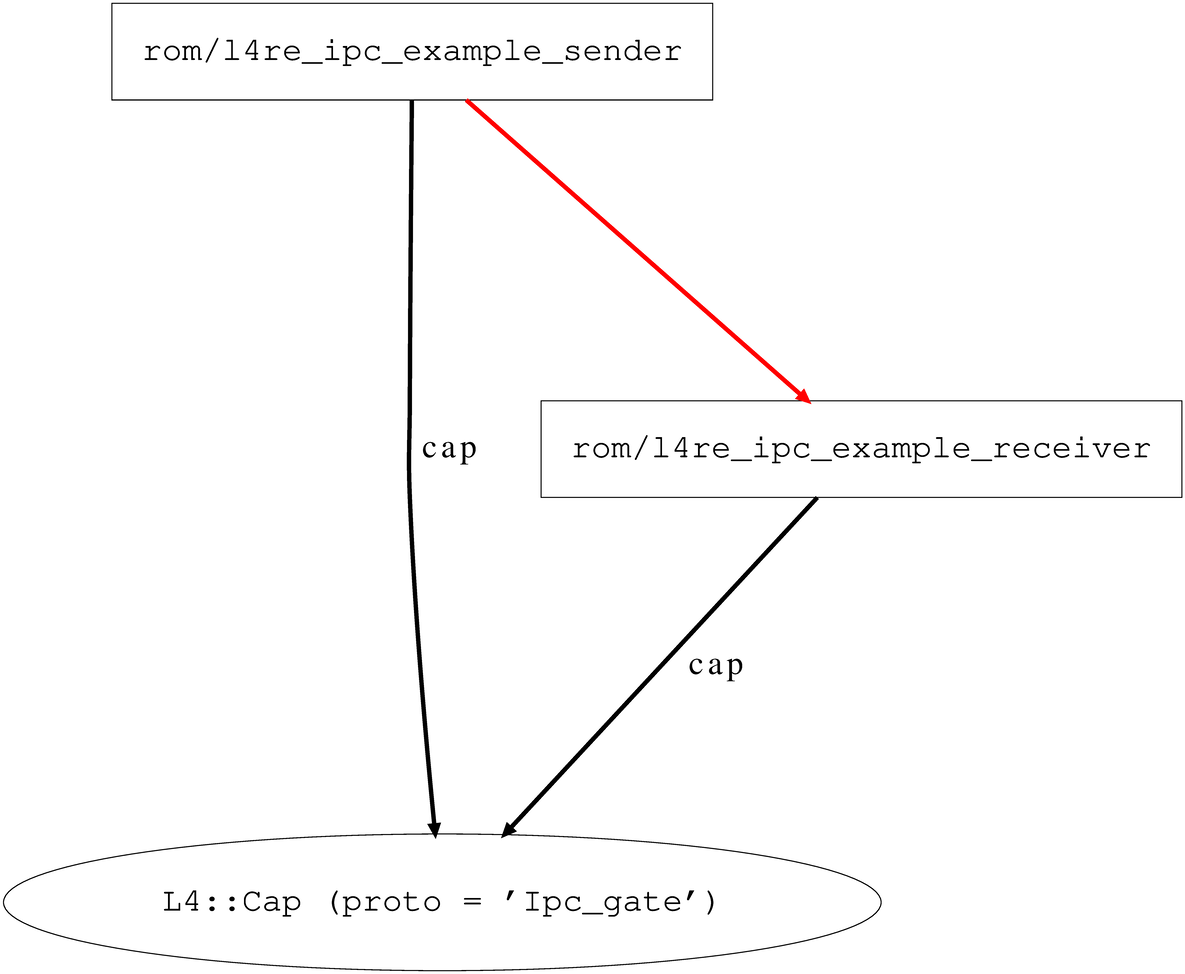
\includegraphics{../resources/nedmock.png}
  \caption{Kommunikations-Struktur von \texttt{l4re\_ipc\_example.cfg}}
  \label{fig:nedmock}
\end{figure}

\section{Code-Coverage}

Um die Auswertung von Unit-Tests zu verbessern, sollte automatisierte
Line-Coverage in das existierende Test-System integriert werden.

Das L4Re Build-System unterstützt hauptsächlich den \textit{GNU C Compiler
(gcc)}.  Mit diesem lassen sich Code-Coverage Daten erzeugen, indem zu
analysierende Programme mit speziellen Flags kompiliert und gelinkt werden.
Diese sorgen dafür, dass zunächst in den im Kompilierungs-Schritt erzeugten
Object-Files Maschinen-Code eingebaut wird, der bei Ausführung dafür sorgt,
dass u.a. die Anzahl der Abarbeitungen für jede nicht heraus-optimierte
Quellcode-Zeile in speziellen Datenstrukturen festgehalten wird. Außerdem
werden die Programme gegen zusätzlichen Code gelinkt, der vor Ausführung von
\texttt{main} einen Exit-Handler registriert. In diesem werden gegen Ende des
Programms die in einer statisch allokierten verketteten Liste (mit einem
Listen-Element für jedes Object-File aus dem das ausgeführte Programm erzeugt
wurde) gespeicherten Coverage-Daten in ein binäres Datenformat umgewandelt und
im Dateisystem neben den Quellcode-Dateien, aus denen das Programm erzeugt
wurde, abgelegt. Genau genommen werden pro Quellcode-Datei zwei für die
Generierung von Coverage-Dateien relevante Dateien erzeugt: eine Datei im
\texttt{.gcno} Format wird bereits während des Compilierungs-Schrittes
generiert. Nach Programmausführung entsteht wie beschrieben zusätzlich eine
\texttt{.gcda} Binärdatei. Beide werden benötigt um menschenlesbare
Coverage-Reports zu generieren.

Im Zusammenhang mit L4Re ist hier problematisch, dass die derartige Erzeugung
von Coverage-Daten das Vorhandensein eines Dateisystems voraussetzt.  Diese
Bedingungen ist für die in einer virtuellen Maschine ausgeführten Unit-Tests
nicht gegeben. Vielmehr wäre es wünschenswert, die Daten auf der seriellen
Konsole auszugeben, sodass sie bei Testausführung gegebenenfalls von einem
Wrapper-Skript geparst und im Dateisystem des Host-Systems abgelegt werden
können. Mit dem intern zur Test-Ausführung verwendeten Perl 5 Programm
\textit{Tapper} existierte bereits ein solches Wrapper-Skript, welches bisher
aber nur die bei Ausführung von Tests auf der seriellen Konsole ausgegebenen
Ergebnisse parsen und für den Nutzer in ein ,,angenehmeres'' Format
transformieren konnte.

Die Funktionen zur Ausgabe von Coverage Daten sind in gcc in
\texttt{libgcc/gcov.h} und \texttt{gcc/gcov*} implementiert. Sie lassen sich
durch eine eigene Implementierung ersetzen, indem eine mit
\texttt{-fprofile-arcs} und \texttt{-ftest-coverage} kompilierte Objekt-Datei
gegen eine solche gelinkt wird. Listing~\ref{lst:gcov} zeigt den
,,alternativen'' gcov Exit-Handler, welcher die Coverage-Daten mittels
\texttt{printf} ausgibt anstatt sie in eine Datei zu schreiben. Die Marker
\texttt{GCOV GCDA/DATA/DONE} können später von Tapper erkannt werden. Tapper
schreibt dann die im Hexadezimal-Format ausgegebenen Binärdaten in die
angegebenen \texttt{.gcda} Datei im Host-Dateisystem.

\begin{mintlisting}[label=lst:gcov]{mintc}{Modifizierter gcov Exit-Handler}
static void __attribute__((destructor))
gcov_exit(void)
{
  /* buffer to hold extracted gcda data */
  enum { Buf_sz = 1 << 15 };

  static char output_buffer[Buf_sz];

  /* iterate over the list of coverage data nodes */
  struct gcov_info *tmp = __gcov_master.list_start;

  while (tmp)
    {
      /* dump gcda path */
      printf("GCOV GCDA %s\n", gcov_info_filename(tmp));

      /* dump coverage data */
      size_t buf_sz = convert_to_gcda(NULL, tmp);
      assert(buf_sz < Buf_sz);

      convert_to_gcda(output_buffer, tmp);

      printf("GCOV DATA ");
      for (size_t i = 0; i < buf_sz; ++i)
        printf("%02X", (output_buffer[i] & 0xff));
      putchar('\n');

      /* continue with the next coverage data node */
      tmp = tmp->next;
    }

  printf("GCOV DONE\n");
}
\end{mintlisting}

\section{Benchmarking}

Kernkonzept nutzt eine zu großen Teilen intern entwickelte Pipeline zur
automatisierten Ausführung von Integrations-Tests und Benchmark-Programmen
auf verschiedenen Hardware-Plattformen.
Die gesammelten Benchmark-Ergebnisse werden auf einem zentralen Server
gespeichert und können über ein Web-Frontend dargestellt werden.

Das bisherige Frontend ist hauptsächlich in Perl 5 und JavaScript
geschriebenen. Es erfüllt seinen Zweck, ist aber in manchen Belangen nicht
flexibel genug. Vor allem ist das Einbinden neuer Funktionen teilweise mit
größerem Aufwand verbunden und nur mit ausreichender Kenntnis der
existierenden Software möglich.

Es wurde die Nutzung von \textit{Jupyter} als Alternative evaluiert. Jupyter
ist in Web-Frontend für den \textit{IPython} Kernel (unter anderen) und erlaubt
die Ausführung von Python-Code in einem Zellen-basierten Editor im Browser. In
den so entwickelten sogenannten Notebooks lassen sich neben Python-Code auch
mit gängigen Plotting-Bibliotheken erzeugte Grafiken inline darstellen. Die
Ergebnisse können dann beispielsweise automatisch in verschiedene Formate
exportiert werden, die gängige Browser auch ohne Jupyter Installation
darstellen können.

Die Umstellung der Benchmark-Daten-Visualisierung auf Jupyter bringt vor allem
einen Vorteil mit sich: Es existieren aufgrund der Beliebtheit von Python in
der Data Science Community etliche aktiv entwickelte Open Source Bibliotheken
zur statistischen Analyse und Darstellung von Daten. Dies kann in Zukunft die
Implementierung von spezialisierten Funktionalitäten ersparen, für die die
beispielsweise bereits eine verfügbare Python- aber keine äquivalente
JavaScript-Lösung existiert.

\subsection{Datenanfrage}

Zunächst wurde ein Teil des existierenden Perl 5 Codes, der für die Abfrage der
Benchmark-Daten vom Server verantwortlich ist, nach Python portiert.  Die
Benchmark-Daten werden auf einem Test-Server von in festgelegten Intervallen
geschedulten Jobs erzeugt.  Diese führen teilweise komplexe Integrations-Tests
aus und messen verschiedene Performance-Metriken, z.B. Latenzen beim Versenden
von IP-Paketen zwischen verschiedenen VM Instanzen.

Für die strukturierte Speicherung und Verwaltung dieser Metriken existieren
verschiedene Backend-Implementierungen, u.a. RDBMS oder \textit{Elastisearch}
basiert.  Die Abfrage der Daten ist nach außen über ein JSON basiertes
Interface abstrahiert. Dieses ähnelt gebräuchlichen deklarativen
Anfragesprachen wie etwa SQL ist aber deutlich einfacher gehalten.

Die derart persistierten Daten können vom Server, auf dem sie abgelegt sind,
angefragt werden, indem eine Query im JSON Format per HTTP POST-Anfrage an den
Server übertragen wird. Die zur Anfrage passenden Daten sind in der HTTP
Antwort (im CSV Format) enthalten.

\subsection{Visualisierung}

Um die angefragten Daten darzustellen, wurde eine Python Bibliothek geschrieben,
die häufig anfallende Visualisierungs-Aufgaben einfach macht.  Diese ermöglicht
die direkte Darstellung von Histogrammen, Boxplots, Quantilen etc. direkt mit
den in Python-Objekten gekapselten angefragten Datensätzen. Die Bibliothek
nutzt dabei die Python Plotting Bibliotheken \textit{Matplotlib} und
\textit{Bokeh} als austauschbare Backends und abstrahiert über deren
unterschiedliche APIs. Bokeh erzeugt mittels JavaScript-Generierung interaktive
Plots (mit integrierter Zoom-Funktion usw.), was diese besonders gut in aus
Jupyter Notebooks erzeugten Web-Dokumenten nutzbar macht. Das Matplotlib
Backend wurde zusätzlich implementiert, da Bokeh sich noch in einer frühen
Entwicklungsphase befindet und vor allem bezüglich Dokumentation und
API-Stabilität weniger ausgereift ist. Technisch war hier die sinnvolle
Abstrahierung und Konsolidierung der teilweise sehr ,,grundlegenden'' von Bokeh
und Matplotlib angebotenen Plotting-Funktionen zu einem für den vorliegenden
Anwendungsfall geeigneten ,,high-level'' Interface eine Herausforderung.

\subsection{Regelkarten}

\textit{Regelkarte} ist ein Oberbegriff für verschiedene statistische Methoden,
die genutzt werden können um das ,,Außer-Kontrolle-Geraten'' eines
statistischen Schwankungen unterliegenden Prozesses zu erkennen. Man stelle
sich als Beispiel eine in regelmäßigen Zeitabständen gemessene L4Re
Performance-Metrik vor (zum Beispiel Latenz einer bestimmten Form der
Netzwerk-Kommunikation), für die der ermittelte Wert im Normalfall ungefähr um
einen konstanten Mittelwert normalverteilt ist. Es wäre nun wünschenswert, es
ohne manuelle Inspektion zu ermöglichen, Abweichung von diesem Verhalten, wie
zum Beispiel eine Verschiebung des Mittelwertes, rechtzeitig zu erkennen und
auf gewisse Commits zurückführen zu können. Eine naive Lösung wäre es, einen
cron-Job o.ä. anzulegen, der nach jeder Messung eine Warnung ausgibt, wenn die
ermittelte Metrik einen festen Grenzwert überschreitet. Dies führt dann aber in
den meisten Fällen entweder zu vielen Falschmeldungen, wenn der Grenzwert zu
eng angesetzt ist oder andernfalls zu später (oder gar keiner) Erkennung von
anhaltenden, aber kleinen Abweichungen im Mittelwert oder der
Standardabweichung des Prozesses.

Verschiedene Regelkarten können hier Abhilfe schaffen. Die meisten von ihnen
setzen normalverteilte Prozesse mit bekanntem Mittelwert und Standardabweichung
voraus (die aber auch aus einer Menge von Datenpunkten mit statistischen
Formeln angenähert werden können) und berechnen aus einer Zeitreihe von
Messwerten kumulativ einen Wert, der als Maß für das Außer-Kontrolle-Geraten
des Prozesses genutzt und auf Überschreitung eines Grenzwertes geprüft werden
kann.

Bei \textit{CUSUM} Regelkarten werden so zum Beispiel die akkumulierten Differenzen
zwischen dem Prozess-Mittelwert und dem Sollwert betrachtet, wodurch auch
kleine systematisch Verschiebungen des Mittelwertes detektiert werden können.
Letztlich wurden die Regelkarten-Typen $\bar{x}$ \textit{and R}, $\bar{x}$
\textit{and s}, \textit{ImR}, \textit{XmR}, \textit{EWMA} und \textit{CUSUM} in
die Benchmark-Visualisierungs-Bibliothek aufgenommen. Die genaue
Auseinandersetzung mit einzelner Regelkarten übersteigt den Rahmen dieses
Berichtes, für eine für Nicht-Statistiker zugängliche Einführung in gängige
Regelkarten-Typen siehe~\cite{nist}.

Listing~\ref{lst:control_charts} zeigt Beispielhaft die Erzeugung einer Reihe von
Regelkarten. Per JSON werden hier die zu analysierenden Datenpunkte sowie
Regelkarten-Typen spezifiziert. Bei der Erzeugung der Regelkarten-Objekte werden
die Datenpunkte per HTTP Post-Anfrage an \texttt{TAGET\_BASE\_URL} von einem
Server abgefragt. Schließlich werden die Regelkarten visualisiert, das Ergebnis
zeigt Abbildung~\ref{fig:control_charts}. In diesem Fall ist der Prozess unter
Kontrolle, in allen Regelkarten wird der ,,Kontrollbereich'' (abgegrenzt durch
,,Upper'' und ,,Lower Control Limit'' (UCL und LCL)) nicht verlassen.

\begin{mintlisting}[label=lst:control_charts]{mintpython}{Regelkarten-Visualisierung}
json_data = {
    "TARGET_BASE_URL" : "http://.../api/v1/",
    "METRIC" : {
        "NAME": "l4re.bmk.memory.stream.scale",
        "REF_QUERY": {
           "where" : [["<=", "CREATED", "2018-04-13 00:00:00"]]
        },
        "MONITOR_BASENAME": "MONITOR.processcontrol.ct.stream.x201.l4linux.l4vio_net_p2p",
        "MONITOR_VERSION": 1001,
        "MONITOR_QUERY": {
            "where" : [["=", "l4re_platform_hwcodename", "PCX201A"]]
        },
        "MONITOR_PARAMS" : {},
        "MONITOR_TYPES": [
            "cusum",
            "ewma",
            "xbar_s"
        ],
        "MONITOR_START": "2018-04-01 00:00:01",
        "SUBGROUP_SIZE": 5
    }
}

# create control charts
xbar_s = ControlChart.from_json('xbar_s', json_data)
cusum = ControlChart.from_json('cusum', json_data)
ewma = ControlChart.from_json('ewma', json_data)

# plot control charts
vis = MatplotlibPlotter()

vis.start()
vis.xbar_s(xbar_s, equidistant=True)
vis.cusum(cusum, equidistant=True)
vis.ewma(ewma, equidistant=True)
vis.show()
\end{mintlisting}

\begin{figure}
  \centering
  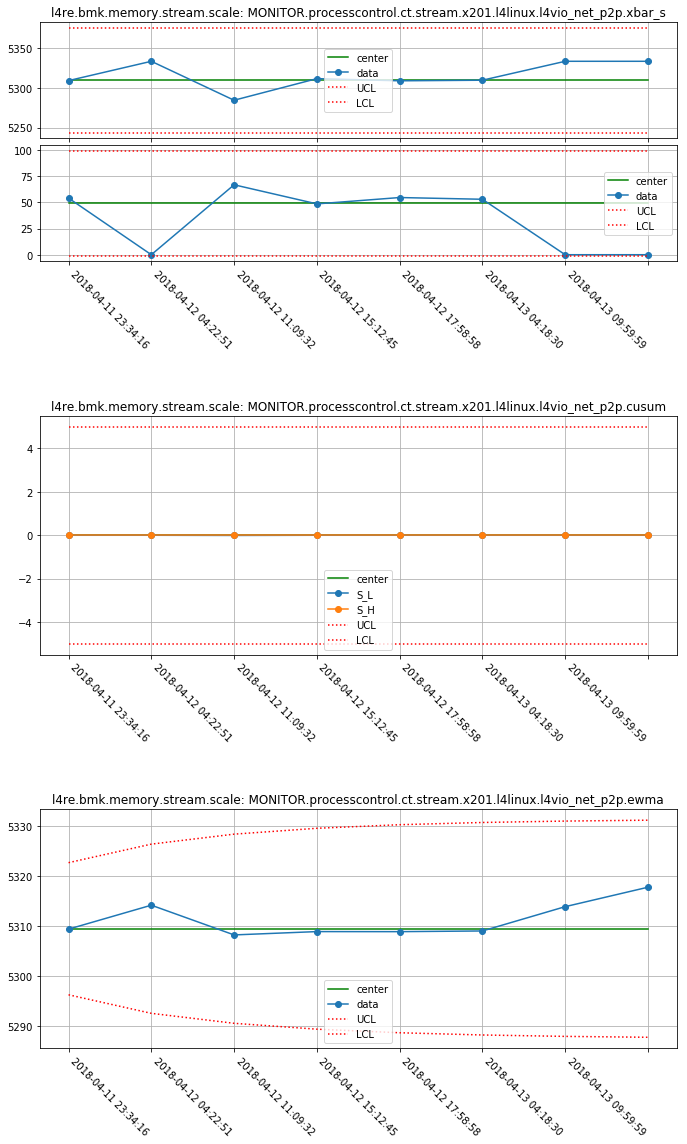
\includegraphics[scale=.6]{../resources/control_charts.png}
  \caption{Regelkarten-Visualisierung}
  \label{fig:control_charts}
\end{figure}

Es wurde zusätzlich ein Python Skript geschrieben, das in regelmäßigen
Abständen die Verfügbarkeit neuer Datenpunkte verschiedener Metriken abfragt,
aus diesen und vorherigen Datenpunkte den nächsten Regelkarten Wert
berechnet, diesen in derselben Datenbank ablegt und bei detektierter Ausartung
des Prozesses eine definierbare Aktion ausführt (sinnvollerweise das
Verschicken einer warnenden Mail).

\section{Gast-Monitor für uvmm}

Mit uvmm ist es möglich, sicher voneinander isolierte virtualisierte
Gast-Systeme (z.B. Linux) auf Fiasco.OC auszuführen. Um den Zustand solcher
Gast-Instanzen zur Laufzeit besser analysieren zu können, sollte ein
,,Gast-Monitor'' entwickelt werden, der es erlaubt, Teile des Zustandes von
Gast-Instanzen über ein \textit{GNU Readline} Interface auszugeben und
gegebenenfalls zu modifizieren. Der Monitor sollte dabei in Release-Builds
keinen Einfluss auf den uvmm Binärcode haben, also durch einfaches Setzen von
Makefile Flags mittels bedingter Kompilierung bereits zur Kompilierzeit
deaktiviert werden können. Der Gast-Monitor implementiert die Ausgabe von:

\begin{itemize}
  \item CPU Zustand (Register etc.)
  \item Speicher-Inhalt
  \item Seitentabellen
  \item Device Tree
  \item Weiterem Architekturspezifischem Systemzustand
\end{itemize}

Abschnitt~\ref{sec:uvmm_monitor_design} beschreibt Design und Implementierung
des Gast-Monitors. Folgende Abschnitte veranschaulichen anhand von Beispielen
die wichtigsten Gast-Monitor Befehle.

\subsection{Design und Implementierung des Gast-Monitors}
\label{sec:uvmm_monitor_design}

Der Gast-Monitor besteht aus zwei Komponenten, die über das \textit{L4::Vcon}
Protokoll kommunizieren: dem ,,CLI Server'' und dem ,,Monitor Interface'' das
Teil von uvmm selbst ist.

\subsubsection{CLI Server}

% TODO: drop in replacement
% TODO: ned example

Der CLI Server ist ein von uvmm unabhängiges L4Re Programm welches ein auf GNU
Readline basiertes Kommandozeilen-Interface implementiert. Gibt der Nutzer
einen Befehl ein, wird ein \textit{virtueller Interrupt (IRQ)} an uvmm gesendet.
uvmm liest daraufhin über das Vcon Protokoll den Befehl + Zeilenumbruch ein,
verarbeitet ihn, und sendet eine oder mehrere Zeilen Ausgabe zurück an den CLI
Server.

Das Ende der Ausgabe wird immer durch die Zeichenkombination EOT +
Zeilenumbruch signalisiert. Der CLI Server gibt seinerseits die von uvmm
erhaltene Ausgabe aus und setzt das Einlesen von Befehlen fort.

Zusätzlich implementiert der CLI Server Befehlsvervollständigung ähnlich wie
z.B. gängige Unix Shells. Hierzu wird bei Eingabe des Tabulatorzeichens die
aktuelle Befehlszeile bis zur Cursorposition + Tabulatorzeichen + Zeilenumbruch
über den zuvor beschriebenen Mechanismus an uvmm gesendet. uvmm ermittelt dann
mögliche Vervollständigungen für das letzte Wort der Befehlszeile und sendet
diese -getrennt durch Zeilenumbrüche und wieder gefolgt von EOT + Zeilenumbruch-
zurück an den CLI Server, der von Readline bereitgestellte Funktionen nutzt um
die aktuelle Befehlszeile automatisch zu vervollständigen.

Der CLI Server setzt sich aus zwei Singleton Klassen zusammen:
\texttt{Readline\_loop} und \texttt{uvmm\_cli\_vcon}. Erstere implementiert
eine Endlosschleife in der mittels Readline Nutzereingabe gelesen wird, sowie
Befehls-Vervollständigung, History-Verwaltung und einige String-Verarbeitungs
Funktionen.  Letztere ist eine von \texttt{L4Re::Util::Vcon\_svr} abgeleitete
Klasse, welche die vererbten Funktionen \texttt{vcon\_read} und
\texttt{vcon\_write} überschreibt, die das Senden/Empfangen von Daten
an/von uvmm implementieren.

Listing~\ref{lst:readline_loop} verdeutlicht die Struktur der in
\texttt{Readline\_loop} implementierten Readline Schleife.

\begin{mintlisting}[label=lst:readline_loop]{mintcpp}{\texttt{Readline\_loop::run} (aus \texttt{uvmm\_cli.cc})}
void Readline_loop::run(char const *prompt)
{
  for (;;)
    {
      // read next command
      char *line = readline(prompt);

      // ...

      // send (preprocessed) command to uvmm
      uvmm_cli_vcon::get()->send(line_preprocessed);

      // print uvmm's response
      std::cout << uvmm_cli_vcon::get()->receive();
    }
}
\end{mintlisting}

\texttt{uvmm\_cli\_vcon} wird vom CLI Server in einen ,,Server Loop''
eingehängt. Der Server Loop realisiert eine high-level Abstraktion der in
Abschnitt~\ref{sec:l4re_pi} eingeführten IPC Mechanismen. Dabei werden die
Interfaces von von \texttt{L4::Epiface} abgeleiteten Objekte zur Laufzeit
anderen Programmen zur Verfügung gestellt. Diese können (z.B. über Ned)
Capabilities auf erstere erhalten und per Remote Procedure Calls (RPCs) deren
Member-Funktionen aufrufen.

Listing~\ref{lst:registry_server} zeigt das Aufsetzen des Server Loops.  Wird
die unter dem Namen \texttt{"mon"} exportierte Capability vom Typ
\texttt{L4::Vcon} von Ned in uvmm hereingereicht, kann uvmm so per
\texttt{uvmm\_cli\_vcon::vcon\_read/write} Daten mit dem CLI Server
austauschen. Man beachte, dass Aufrufe dieser Funktionen im Haupt-Thread des
CLI-Servers abgehandelt werden, während die Readline Schleife in einem
Neben-Thread läuft.

\begin{mintlisting}[label=lst:registry_server]{mintcpp}{CLI Server Server Loop}
// start readline thread
std::thread readline_thread(run_readline, "monitor> ");

// create registry
L4Re::Util::Registry_server<L4Re::Util::Br_manager_hooks> registry_server;

registry_server.registry()->register_obj(uvmm_cli_vcon::get(), "mon");

// start server loop
registry_server.loop();
\end{mintlisting}

Der Austausch von Daten zwischen dem CLI server und uvmm erfolgt über zwei
Puffer, \texttt{uvmm\_cli\_vcon::\_send\_buf} und
\texttt{uvmm\_cli\_vcon::\_receive\_buf}.  \texttt{uvmm\_cli\_vcon::send}
beschreibt den Sende-Puffer der von uvmm mittels
\texttt{uvmm\_cli\_vcon::vcon\_read} ausgelesen wird. Umgekehrt schreibt uvmm
mittels \texttt{uvmm\_cli\_vcon::vcon\_write} Daten in den Empfangs-Puffer,
welcher mittels \texttt{uvmm\_cli\_vcon::receive} ausgelesen wird.  Um diesen
Ablauf zu realisieren, müssen einige Synchronisations-Vorkehrungen getroffen
werden um Race-Conditions u.ä vorzubeugen.

Da der Zugriff auf beide Puffer sowohl vom Readline Thread als auch asynchron
(ausgelöst von uvmm) im Haupt-Thread  erfolgt, müssen Zugriffe auf diese mit
Mutexen synchronisiert werden.  Weiterhin ist es wünschenswert, dass
\texttt{send} solange blockiert, bis uvmm mit der gesamten Ausgabe geantwortet
hat. So wird garantiert, dass uvmm immer maximal einen Befehl zur Zeit
abarbeitet, was die Implementiertung des Monitor Interface vereinfacht. Nach
Rückkehr von \texttt{send}, kann demnach auch uvmms Ausgabe sofort mittels
einem nicht-blockierenden Aufruf von \texttt{receive} ausgelesen werden.  Dies
ist mittels einer Semaphore implementiert, die in \texttt{send} dekrementiert
und in \texttt{vocn\_write} wieder inkrementiert wird wenn die gesamte Ausgabe
von uvmm empfangen worden ist.

Listing~\ref{lst:uvmm_cli} zeigt vereinfachte Darstellungen von \texttt{send},
\texttt{receive}, \texttt{vcon\_read} und \texttt{vcon\_write}, die diesen
Prozess veranschaulichen. Man beachte, dass dieser vor allem dadurch
kompliziert wird, dass uvmm den Sende- bzw. Empfangs-Puffer nicht zwangsweise
,,auf einmal'' (nicht einmal zeilenweise) liest/beschreibt. Die Variable
\texttt{\_ready\_to\_receive} ist immer dann gesetzt, wenn
\texttt{uvmm\_cli\_vcon} uvmm Ausgabe erwartet. Damit wird verhindert, dass
verirrte Aufrufe von \texttt{vcon\_write} durch uvmm während des Sendens eines
Befehls oder nach Empfangen der Ausgabe den Empfangs-Puffer verändern.

\begin{mintlisting}[label=lst:uvmm_cli]{mintcpp}{\texttt{uvmm\_cli\_vcon} Vcon Interface (aus \texttt{uvmm\_cli.cc})}
// uvmm requests to read 'size' characters into 'buf'
unsigned uvmm_cli_vcon::vcon_read(char *buf, unsigned size)
{
  std::lock_guard<std::mutex> lock(_send_mutex);

  if (_send_buf.empty())
    return L4_VCON_READ_STAT_DONE; // signal to uvmm that there is no more to read

  if (size == 0)
    return 0; // ignore read requests of size zero

  if (size < _send_buf.size())
    {
      // send the first 'size' characters of '_send_buf'
      memcpy(buf, _send_buf.data(), size);
      _send_buf = _send_buf.substr(size);
    }
  else
    {
      // uvmm wants to read all available characters

      // send every character in '_send_buf'
      memcpy(buf, _send_buf.data(), _send_buf.size());

      // signal to uvmm that there is not more to read
      size = _send_buf.size() | L4_VCON_READ_STAT_DONE;

      _send_buf.clear();
      _ready_to_receive = true;
    }

  return size;
}

// uvmm requests to write 'size' characters from 'buf'
void uvmm_cli_vcon::vcon_write(const char *buf, unsigned size)
{
  if (!_ready_to_receive)
    return; // ignore request if there is still a 'send' in progress

  if (size == 0)
    return; // return write requests of size zero

  std::lock_guard<std::mutex> lock(_receive_mutex);

  // check whether output sent by uvmm contains the EOT character...
  char const *eot = static_cast<char const *>(memchr(buf, (char)uvmm_cli::PROTO_EOT, size));

  if (eot)
    {
      // ...if so, we have received the complete output...
      _receive_buf << std::string(buf, eot);
      _ready_to_receive = false;

      // ...and can thus unblock 'send' so the next command can be sent to uvmm
      _sem->up();
    }
  else
    {
      _receive_buf << std::string(buf, buf + size);
    }
}

// send the command in 'buf' to uvmm
void uvmm_cli_vcon::send(std::string const &buf)
{
  {
    std::lock_guard<std::mutex> lock(_send_mutex);

    _send_buf = buf + '\n';
  }

  // signal uvmm to start reading the command
  _irq.trigger();

  // block until the command's output has been returned by uvmm
  _sem->down();
}

std::string uvmm_cli_vcon::receive()
{
  std::lock_guard<std::mutex> lock(_receive_mutex);

  std::string ret(_receive_buf.str());

  // clear the receive buffer
  _receive_buf.str("");

  return ret;
}
\end{mintlisting}

Listing~\ref{lst:uvmm_cli_ned} zeigt schließlich ein Ned-Skript mit dem uvmm
sowie der CLI Server gestartet und verbunden werden können. Über das
Hilfs-Module \texttt{vmm} wird eine uvmm Instanz mit einem Linux Gast (mit
Kernel Image \texttt{bzImage}) gestartet. Durch das modulare Design ist es
denkbar, den CLI Server durch ein beliebiges anderes L4Re Programm zu ersetzen,
das über das gleiche Protokoll mit uvmms Monitor Interface kommuniziert.

\begin{mintlisting}[label=lst:uvmm_cli_ned]{mintlua}{Ein Gast-Monitor Ned-Skript}
local l4 = require 'l4'
local l = l4.default_loader

local vmm = require 'vmm'

mon = l:new_channel()

vmm.start_vm
  {
    id       = 1,
    mem      = 196,
    kernel   = 'rom/bzImage',
    bootargs = 'console=hvc0 ramdisk_size=13000 root=/dev/ram1 nokaslr',
    rd       = 'rom/ramdisk.rd',
    fdt      = 'rom/virt-pc.dtb',
    cpus     = 1,
    mon      = mon
  }

l:start
  (
    { caps = { mon = mon:svr() } },
    "rom/uvmm_cli"
  )
\end{mintlisting}

\subsubsection{Monitor Interface}

Auf uvmm Seite ist das Monitor-Interface über eine Reihe von ,,Command
Handler'' Klassen realisiert. Diese Klassen greifen auf für den Gast-Monitor
interessante Daten und Funktionen uvmm interner Klassen zu. Jeder Command
Handler ist eine Klassen-Template, welche über Vererbung mit einer
entsprechenden uvmm Klasse verknüpft ist. Am Beispiel der fiktiven Klasse
\texttt{X}:

\begin{mintlisting}{mintcpp}{Aufbau eines Command Handlers}
namespace Monitor {

enum : bool {
#ifdef CONFIG_MONITOR
  Enabled = true,
#else
  Enabled = false,
#endif
}

template<bool, typename T>
class X_cmd_handler {};

template<typename T>
class X_cmd_handler<true, T> : public Cmd
{
  // ...

  X *x()
  { return static_cast<T *>(this); }

  X const *x() const
  { return static_cast<T const *>(this); }
};

}

class X : private Monitor::X_cmd_handler<Monitor::Enabled, X>
{
  friend X_cmd_handler<Monitor::Enabled, X>;

  // ...
};
\end{mintlisting}

Dieses Design hat einige Vorteile:

\begin{itemize}
  \item Ist \texttt{CONFIG\_MONITOR} zur Übersetzungszeit nicht definiert,
        erbt \texttt{X} von einer leeren Klassen welche daher dank
        \textit{empty base optimization} vom Compiler komplett
        wegoptimisiert werden kann.
  \item Es muss zur Laufzeit nicht für jedes instanziierte Objekt vom Typ
        \texttt{X} ein separates Objekt vom Typ \texttt{X\_cmd\_handler}
        Objekt instanziiert und mit ersterem verknüpt werden.
  \item \texttt{X\_cmd\_handler} kann auf alle Member von \texttt{X} zugreifen
        (per \texttt{x()->...}).
\end{itemize}

\texttt{Monitor::Cmd} ist eine abstrakte Klasse, die das Interface definiert,
das ein Command Handler implementieren muss um einen Monitor Befehl zu
realisieren. Dazu gehören insbesondere \texttt{Cmd::exec} und
\texttt{Cmd::complete}, welche die bei Ausführung und Vervollständigung eines
Monitor Befehls ausgeführten Aktionen implementieren.  Über
\texttt{Cmd::register\_toplevel} kann ein Command Handler sich in seinem
Konstruktor zudem unter einem Namen in eine uvmm interne Tabelle eintragen.
Empfängt uvmm einen Monitor Befehl, wird dann in dieser Tabelle nach einem
entsprechenden Command Handler gesucht und dessen \texttt{exec} Funktion
aufgerufen.  Dies geschieht immer dann, wenn uvmm einen IRQ vom CLI Server
empfängt. Der IRQ wird von der IRQ Endpoint Klasse \texttt{Cmd\_control}
abgehandelt, die auch die \texttt{L4::Vcon} Capability hält, über die mit dem
CLI Server kommuniziert wird. Listing~\ref{lst:cmd_control} skizziert diesen
Prozess.

\begin{mintlisting}[label=lst:cmd_control]{mintcpp}{Befehls-Ausführung auf uvmm Seite per \texttt{Cmd\_control}}
class Cmd_control : public L4::Irqep_t<Cmd_control>
{
public:
  // ...
  Cmd_control()
  : _con(L4Re::Env::env()->get_cap<L4::Vcon>("mon"))
  {}

private:
  // ...
  L4::Cap<L4::Vcon> _con;
}

void Cmd_control::bind(L4::Registry_iface *registry)
{ _con->bind(0, registry->register_irq_obj(this)); }

void Cmd_constrol::handle_irq()
{
  std::string cmdline;
  if (!get_line(&cmdline)) // uses _con->read
    return;

  handle_cmd(cmdline);
}

void Cmd_control::handle_cmd(std::string const &cmdline)
{
  Monitor::Cmd *handler = find_cmd_handler(cmdline);

  if (!handler) {
    fprintf(_f, "Monitor: Unknown cmd %.*s\n", cmd_line);
    return;
  }

  Monitor::Arglist arglist(cmdline); // utility argument stack

  // execute command, all command output should be written to the the file
  // handle _f, arglist allows retrieving (typed) command arguments in order
  handler->exec(_f, &arglist);
}
\end{mintlisting}

Nicht alle Command Handler müssen \texttt{register\_toplevel} aufrufen. Einige
von ihnen implementieren vielmehr ,,Unter-Befehle''. Ihre \texttt{exec}
Funktionen werden direkt von einem übergeordneten Command Handler aufgerufen.

\subsection{CPU-Zustand}

uvmm unterstützt eine Reihe von Host/Gast Architekturen. Einige Teile von uvmms
Quellcode sind daher architekturspezifisch. Der Quellcode ist
wie in Listing~\ref{lst:uvmm_tree} dargestellt aufgebaut:

\begin{mintlisting}[label=lst:uvmm_tree]{minttext}{uvmm Verzeichnisstruktur}
uvmm
  server
    src
      ARCH-amd64
        // architektureabhängige Quellcode-Dateien
        monitor
      // weite Architektur-Verzeichnisse
      debugger
      monitor
      // architektureunabhängige Quellcode-Dateien
\end{mintlisting}

Die \texttt{ARCH-*} Verzeichnisse enthalten architekturspezifischen Code.
Beispielsweise enhalten alle von ihnen eine Implementierung der Klasse
\texttt{Cpu\_dev}, definiert in \texttt{Arch-*/cpu\_dev.h/cc} welche den
Zustand einer Gast-CPU abstrahiert. Alle diese Klassen erben ihrerseits
architekturunabhängige Funktionalität von \texttt{Generic\_cpu\_dev} definiert
in \texttt{generic\_cpu\_dev.hpp}. Zur Kompilierzeit wird über die Makefile
Variable \texttt{ARCH} kontrolliert welche \texttt{cpu\_dev.h/cc} Variante
kompiliert und mit dem restlichen Code gelinkt wird.

Das Monitor Interface integriert nach demselben Prinzip architekturunabhängigen
und architekturspezifischen Quellcode, z.B. die Klassen \texttt{Cpu\_dev\_cmd\_handler} (in \texttt{ARCH-*/monitor/cpu\_dev\_cmd\_handler.h} und \texttt{Cpu\_dev\_array\_cmd\_handler} (in
\texttt{monitor/cpu\_dev\_array\_cmd\_handler.h}).

Letztere implementiert den in Listing~\ref{lst:cpu_cmd} gezeigten Befehl.
So kann dann etwa mit \texttt{cpu 0 regs} der Unterbefehl \texttt{regs},
welcher die Ausgabe des aktuellen CPU-Register-Zustandes bewirkt, an die
erste Gast-CPU weiteregeleitet werden. Dieser Unterbefehl wird dann von
\texttt{Cpu\_dev\_cmd\_handler} abgearbeitet. Welche Unterbefehle verfügbar
sind ist demnach architekturabhängig, z.B. kann unter x86 zusätzlich zu den
Standard-CPU-Registern \textit{Virtual Machine Extensions (VMX)} spezifischer
Zustand mittels \texttt{cpu <i> vmx} ausgegeben werden wie in Listing~\ref{lst:cpu_cmd} demonstriert.

\begin{mintlisting}[label=lst:cpu_array_cmd]{minttext}{\texttt{cpu} Monitor Befehl}
~\color{red}{monitor>}~ help cpu
CPU state
* 'cpu list': list available CPUs
* 'cpu <i> <subcmd>': execute <subcmd> for CPU <i>
\end{mintlisting}

\begin{mintlisting}[label=lst:cpu_cmd]{minttext}{x86 \texttt{cpu} Unterbefehle}
~\color{red}{monitor>}~ cpu 0 regs
RAX ffffffff819b9ec0
RBX 0
RCX 6e0
RDX 1f
RSI 202c2523
RDI 46
RSP 0
RBP 0
R8 0
R9 ffffffff822507c0
R10 ffffffff8224f540
R11 18
R12 ffffffff8280e900
R13 ffffffff828162e0
R14 0
R15 0
RIP ffffffff819ba051
~\color{red}{monitor>}~ cpu 0 vmx
(C) VPID: 0x0
(C) Int notification vector: 0x0
(C) EPTP index: 0x0
(C) EPT pointer: 0x0
...
\end{mintlisting}

\subsection{RAM}

Mit dem \texttt{ram} Monitor Befehl lässt sich der von uvmm verwaltete Speicher
untersuchen. Dieser beinhaltet den gesamten physischen Gast Speicher.
Listing~\ref{lst:ram_cmd} zeigt den Gebrauch dieses Befehls. Der angegebene
Dataspace ist der physische Gast Speicher der an Adresse \texttt{0x01200000} in
uvmms virtuellen Adressraum gemappt ist. Der nachfolgende \texttt{dump}
Unterbefehl gibt die ersten 80 in diesem gespeicherten Bytes aus.

\begin{mintlisting}[label=lst:ram_cmd]{minttext}{\texttt{ram} Monitor Befehl}
~\color{red}{monitor>}~ help ram
Usage:
* ram ds: List RAM dataspaces
* ram dump <addr> [<n> [(b|w|d|q)]]: Dump RAM region
where: * b = byte, w = word, d = double word, q = quad word
       * <n> = number of entries to be dumped
~\color{red}{monitor>}~ ram ds
Dataspace  Guest area             Size        Local address  Phys?
       23  0x00000000-0x0c400000  0x0c400000  0x01200000     Y
~\color{red}{monitor>}~ ram dump 0x01200000 10 q
0x0000000001200000: 0xf668408b48000003
0x0000000001200008: 0x2444c64174026040
0x0000000001200010: 0x4c00000002be0257
0x0000000001200018: 0x0004bd4150247c8d
0x0000000001200020: 0x8bfffffea1e90000
0x0000000001200028: 0x830f044539182444
0x0000000001200030: 0xfffee4e9fffffeb2
0x0000000001200038: 0x8d4c00000001beff
0x0000000001200040: 0x000002bd4150247c
0x0000000001200048: 0x02befffffe7ae900
\end{mintlisting}

\subsection{Seitentabellen}

Ein weiteres Feature des Gast-Monitors ist die Möglichkeit,
die Seitentabellen-Auflösung des Gast-Systems darzustellen.

Hierfür muss teilweise auf virtualisierte Gast-Register zugegriffen werden.
Die L4Re vCPU API implement auf Kernel Threads basierte virtuelle Prozessoren.
Neben Virtualisierung werden diese z.B. auch für die Implementierung von
User-Space Threads genutzt. Der Zustand jeder vCPU wird durch eine Objekt vom
Typ \texttt{l4\_vcpu\_state\_t} beschrieben. uvmm verwaltet pro Gast-CPU ein
Objekt vom (architekturspezifischen) Typ \texttt{Vmm::Vcpu\_ptr} welches selbst
ein dünner Wrapper um einen Zeiger auf ein \texttt{l4\_vcpu\_state\_t} Objekt
ist.  So können uvmm Klassen über \texttt{Vmm::Vcpu\_ptr} u.a. auf von Fiaso
zur Verfügung gestellte Gast-Register zugreifen.

Zudem ist es notwendig, in den Seitentabellen gespeicherte physische Gast- in
virtuelle Host-Adressen übersetzen zu können. uvmm verwaltet Gast-Speicher über
sogenannte \textit{Regionen}. Es werden verschiedene Arten von Regionen
unterschieden, solche vom Typ \texttt{Vmm::Region\_type::Ram} bilden
kontinuierliche Adressbereiche im physischen Speicher eines Gasts ab.

Die Klasse \texttt{Vm\_mem} erlaubt es mittels der Funktion
\texttt{Vm\_mem::find\_ram\_region} die zu einer physischen Gast-Adresse
gehörige Region, sowie die Adresse an der diese in uvmms virtuellen
Adressraum abgebildet ist, zu ermitteln. Auf \texttt{Vm\_mem} aufbauend
implementiert \texttt{Cached\_gphys\_to\_hvirt} die effiziente Übersetzung von
pyhsischen Gast Adressen in virtuelle Host Adressen: Liegt eine Adresse in
derselben Region wie die zuvor angefragte, reduziert sich die Übersetzung auf
eine einfache Interpolation vom dieser Region zugehörigen physischen
Gast-Speicher Bereich in den zugehörigen virtuellen Host-Speicher Bereich wie
in Listing~\ref{lst:cached_gphys_to_hvirt} dargestellt.

\begin{mintlisting}[label=lst:cached_gphys_to_hvirt]{mintcpp}{\texttt{Cached\_gphys\_to\_hvirt::lookup}}
int Cached_gphys_to_hvirt::lookup(l4_addr_t gphys, l4_addr_t *hvirt)
{
  Guest_addr ga(gphys);

  if (_cached_start.get() == -1U || _cached_start > ga || _cached_end < ga)
    {
      Ds_handler *ds_handler;

      int err = _mmap->find_ram_region(ga, &_cached_start, &_cached_end, &ds_handler);

      if (err < 0)
        return err;

      _cached_ds_local_start = ds_handler->local_start();
    }

  *hvirt = _cached_ds_local_start + (ga - _cached_start);

  return L4_EOK;
}

\end{mintlisting}

Der Einfachheit halber soll hier nur die Adressübersetzung für x86\_64 im 64
Bit \textit{Long Mode} betrachtet werden\footnote{Die Adressübersetzung im 32
Bit \textit{Protected Mode} funktioniert ähnlich, unterscheidet sich aber in
Details wie z.B. der unterstützten Seitengrößen.}. Die x86\_64 Architektur
implementiert Hardware-unterstützte virtuelle Adressräume über mehrstufige
Seitentabellen. Dafür muss das \textit{Paging (PG)} Bit im Kontrollregister
\texttt{CR0} gesetzt sein.

Obwohl im Long Mode 64 Bit zur Adressierung des virtuellen Adressraumes zur
Verfügung stehen, unterstützen gängige Prozessoren lediglich $2^{48}$ Byte =
256 TiB große virtuelle Adressräume. Bits 48 bis 63 jeder virtuellen Adresse
sind dabei immer gleich Bit 47, so dass gültige virtuelle Adressen trotzdem
eindeutig sind.  Die Standard-Seitengröße ist 4 KiB. Es ist jedoch auch möglich
(falls von der Hardware unterstützt) den Prozessor so zu konfigurieren, dass 2
MiB, oder 1 GiB Seiten verwendet werden.

Der Übersetzungsprozess ist für 4 KiB Seiten vierstufig, für 2 MiB Seiten
dreistufig und für 1 GiB Seiten zweistufig. Die dabei verwendeten Tabellen
werden in der letzten Übersetzungsstufe meist als Seitentabellen und in
vorangehenden Übersetzungsstufen als Seitenverzeichnisse bezeichnet.
Tabelle~\ref{tbl:x86_pt_names} führt die gebräuchlichen konkreten Bezeichnungen
für die vier x84\_64 Seitenverzeichnisse/-tabellen auf\footnote{Diese sind
historisch bedingt, vergleiche z.B. \url{https://www.pagetable.com/?p=14}.}.

\begin{table}[H]
  \centering
  \caption{Bezeichnungen für x86\_64 Seitenverzeichnisse/-tabellen}
  \label{tbl:x86_pt_names}
  \vspace{10pt}
  \label{tbl:page_directory_table_names}
  \rowcolors{2}{}{gray!10}
  \begin{tabular}{rl}
    \toprule
    Stufe & Bezeichnung \\
    \midrule
    1 & \textit{Page Map Level 4 (PML4)} \\
    2 & \textit{Page Directory Pointer Table (PDP)} \\
    3 & \textit{Page Directory Table (PD)} \\
    4 & \textit{Page Table (PT)} \\
    \bottomrule
  \end{tabular}
\end{table}

Die Seitenverzeichnisse/-tabellen liegen im Hauptspeicher und bestehen aus 64-Bit
Einträgen von denen die oberen Bits die physische Adresse eines/einer
folgenden Seitenverzeichnisses/-tabelle bzw. einer Seite bilden.  Die unteren
neun Bits zeigen verschiedene Seiten-Attribute an, wie in
Tabelle~\ref{tbl:page_table_entry_bits} erläutert.  Die
Seitenverzeichnisse/-tabellen werden über Bitfelder in der virtuellen Adresse
indiziert wie in Abbildung~\ref{fig:pt_vaddr} dargestellt. Die unteren Bits der
virtuellen Adresse bilden einen Offset in die Seite selbst.

\begin{table}
  \centering
  \caption{x86\_64 Seiten-Attribute}
  \vspace{10pt}
  \label{tbl:page_table_entry_bits}
  \rowcolors{2}{}{gray!10}
  \begin{tabularx}{\linewidth}{rlX}
    \toprule
    Bit & Bezeichung & Beschreibung \\
    \midrule
    0 & \textit{Present} &
    Die Seite befindet sich im Hauptspeicher (d.h. sie ist nicht etwa in den
    Hintergrundspeicher ausgelagert). Ist dieses Bit beim Zugriff auf eine Seite
    nicht gesetzt, wird ein Seitenfehler ausgelöst.\vspace{\baselineskip} \\
    1 & \textit{Read/Write} &
    Ist dieses Bit gesetzt, kann die Seite von User-Mode Code beschrieben werden%
    \footnote{Kernel-Mode Code hat immer Schreibrechte es sei denn das
    \textit{Write Protect (WP)} Bit in \texttt{CR0} ist gesetzt.}.\vspace{\baselineskip}  \\
    2 & \textit{User/Supervisor} &
    Ist dieses Bit nicht gesetzt, kann nur Kernel-Mode auf die Seite zugreifen.\vspace{\baselineskip}  \\
    3 & \textit{Write-Through} &
    Ist dieses Bit gesetzt, werden Änderungen an der Seite sofort in den
    Hauptspeicher geschrieben.\vspace{\baselineskip}  \\
    4 & \textit{Cache Disable} &
    Ist dieses Bit gesetzt wird die Seite nicht gecached.\vspace{\baselineskip} \\
    5 & \textit{Accessed} &
    Der Prozessor setzt dieses Bit wenn lesend oder schreibend auf die Seite
    zugegriffen wird. Das Betriebssystem ist dafür verantwortlich, dieses Bit
    zurückzusetzen.\vspace{\baselineskip}  \\
    6 & (Nur Seitentabellen) \textit{Dirty} &
    Wie Accessed aber nur für schreibende Zugriffe.\vspace{\baselineskip}  \\
    7 & (Nur Seitenverzeichnisse) \textit{Page Size} &
    Bei 2 MiB/1 GiB großen Seiten ist dieses Bit im Seitenverzeichnis der
    dritten/zweiten Stufe gesetzt.\vspace{\baselineskip}  \\
    8 & (Nur Seitentabellen) \textit{Global} &
    Als Global markierte Seiten werden nicht aus
    dem \textit{Translation Lookaside Buffer (TLB)} geflusht wenn das
    Kontrollregister \textit{CR3} modifiziert wird (typischerweise bei einem
    Kontextwechsel).\vspace{\baselineskip} \\
    \bottomrule
  \end{tabularx}
\end{table}

\begin{figure}
  \begin{bytefield}[endianness=big,bitformatting={\small},bitwidth=.5em,bitheight=8ex]{64}
    \begin{rightwordgroup}{4 KiB Seiten}
        \bitheader{63, 48, 39, 30, 21, 12, 0} \\
        \bitbox{16}{= 47}
        \bitbox{9}{PML4}
        \bitbox{9}{PDP}
        \bitbox{9}{PD}
        \bitbox{9}{PT}
        \bitbox{12}{Offset in Seite}
    \end{rightwordgroup}
  \end{bytefield}

  \vspace{1cm}

  \begin{bytefield}[endianness=big,bitformatting={\small},bitwidth=.5em,bitheight=8ex]{64}
    \begin{rightwordgroup}{2 MiB Seiten}
        \bitheader{63, 48, 39, 30, 21, 0} \\
        \bitbox{16}{= 47}
        \bitbox{9}{PML4}
        \bitbox{9}{PDP}
        \bitbox{9}{PD}
        \bitbox{21}{Offset in Seite}
    \end{rightwordgroup}
  \end{bytefield}

  \vspace{1cm}

  \begin{bytefield}[endianness=big,bitformatting={\small},bitwidth=.5em,bitheight=8ex]{64}
    \begin{rightwordgroup}{1 GiB Seiten}
        \bitheader{63, 48, 39, 30, 0} \\
        \bitbox{16}{= 47}
        \bitbox{9}{PML4}
        \bitbox{9}{PDP}
        \bitbox{30}{Offset in Seite}
    \end{rightwordgroup}
  \end{bytefield}
  \caption{Aufbau einer virtuellen Adresse auf x86\_64}
  \label{fig:pt_vaddr}
\end{figure}

Der vollständige Übersetzungsprozess für eine beliebige virtuelle Adresse
$\mathtt{A_{virt}}$ läuft demnach folgendermaßen ab:

Die Basis-Adresse des ersten Seitenverzeichnisses wird an den oberen Bits des
Kontrollregisters \texttt{CR3}, dem \textit{Page Directory Base Register
(PDBR)}) abgelesen.  Der entsprechende Eintrag $\mathtt{E_{PML4}}$ befindet
sich an Adresse $\mathtt{PDBR} + \mathtt{A_{virt}[PML4]}$.  Ist in diesem das
Present Bit nicht gesetzt, wird ein Seitenfehler ausgelöst. Ansonsten wird die
Basis-Adresse des zweiten Seitenverzeichnisses als $\mathtt{E_{PML4}[12:M-1]} +
\mathtt{A_{virt}[PDP]}$\footnote{\texttt{M} ist hier prozessorabhängig.}
bestimmt.

Dieser Prozess setzt sich fort, bis man entweder im vierten Übersetzungsschritt
bei der Seitentabelle angekommen ist oder in einem Seitenverzeichnis-Eintrag
das Page Size Bit gesetzt ist. In beiden Fällen setzt sich die physische
Adresse dann aus den oberen Bits des Seitentabellen-Eintrages und den bisher
ungenutzen unteren Bits der virtuellen Adresse zusammen.

Listing~\ref{lst:pt_level_next} zeigt vereinfacht die Implementierung dieses
Übersetzungsprozesses. Man beachte, dass in jedem Übersetzungsshritt von
\texttt{Cached\_gphys\_to\_hvirt} Gebrauch gemacht wird, um die aus den
Seitenverzeichnisse/-tabellen ausgelesenen physischen Gast-Adressen in
virtuelle Host-Adressen umzuwandeln.

\begin{mintlisting}[label=lst:pt_level_next]{mintcpp}{Von einem Seitenverzeichnis zum nächsten}
l4_addr_t Pt_walker::gphys_to_hvirt(l4_addr_t gphys)
{
  l4_addr_t hvirt;
  L4Re::chksys(_cached_gphys_to_hvirt.lookup(gphys, &hvirt),
               "Translate guest physical to host virtual address");
  return hvirt;
}

Vmm::Pt_walker::Level Vmm::Pt_walker::Level::next() const
{
  // if we are at the last stage of the lookup, Level::resolve_addrs() has to
  // be called instead in order to retrieve the resolved address
  if (_pt_level == 4 || (_pt_level > 1 && (_pt_entry & Page_size_bit)))
    L4Re::chksys(-L4_EINVAL, "Level is not a leaf");

  l4_uint64_t pt_base_next =
    _pt_level == 0 ? _pt_walker->gphys_to_hvirt(_pt_entry & ~Cr3_pcd_pwt_mask) :
    _pt_walker->gphys_to_hvirt(_pt_entry & _pt_walker->_phys_addr_mask_4k);

  l4_uint64_t pt_index_next =
     _pt_level == 0 ? __virt_addr.pml4() :
     _pt_level == 1 ? __virt_addr.pdpt() :
     _pt_level == 2 ? __virt_addr.pd() :
     _virt_addr.pt();

  l4_uint64_t pt_entry_next = reinterpret_cast<l4_uint64_t *>(pt_base_next)[pt_index_next];

  return Level(/* ... */);
}

void Pt_walker::Level::resolve_addrs(l4_uint64_t *gphys, l4_uint64_t *hvirt)
{
  l4_uint64_t base_addr, offset;

  switch (_pt_level)
    {
    case 2:
      base_addr = _pt_entry & _pt_walker->_phys_addr_mask_1g;
      offset = _virt_addr.raw & G1_offset_mask;
      break;
    case 3:
      base_addr = _pt_entry & _pt_walker->_phys_addr_mask_2m;
      offset = _virt_addr.raw & M2_offset_mask;
      break;
    default:
      base_addr = _pt_entry & _pt_walker->_phys_addr_mask_4k;
      offset = _virt_addr.raw & K4_offset_mask;
      break;
    }

  *gphys = base_addr + offset;
  *hvirt = _pt_walker->gphys_to_hvirt(*gphys);
}
\end{mintlisting}

Listing~\ref{lst:pt_example_x86} zeigt die Anwendung des zugehörigen Command
Handlers. Dieser nutzt intern \texttt{Vmm::Pt\_walker} um eine gegebene
virtuelle Gast-Adresse Schritt für Schritt zu übersetzen und gibt dabei in jedem
Schritt alle für den Übersetzungsprozess relevante Informationen aus. Damit wird
es z.B möglich manuell mittels Assembly Code in einem Gast aufgesetzte
Übersetzungs-Schemata ,,live'' zu debuggen.

\begin{mintlisting}[label=lst:pt_example_x86]{minttext}{\texttt{pt} Monitor Befehl (x86\_64)}
~\color{red}{monitor>}~ help pt
Usage:
* pt: Display page table walk
~\color{red}{monitor>}~ pt ffffffff8107bbb0
CR3:
|Page Directory Base (52)|...|PCD|PWT|...|
|         0x000000000b302|...|  0|  0|...|

Page table @ 0x000000000c502000, entry 511:
|Base (52)      |USR|G|0|0|A|C|W|U|R|P|
|0x0000000002216|000|0|0|1|1|0|0|1|1|1|

Page table @ 0x0000000003416000, entry 510:
|Base (52)      |USR|G|0|0|A|C|W|U|R|P|
|0x0000000002217|000|0|0|1|1|0|0|0|1|1|

Page table @ 0x0000000003417000, entry 8:
|Base (52)      |USR|G|0|0|A|C|W|U|R|P|
|0x0000000001000|000|0|1|1|1|0|0|0|1|1|

Guest physical address: 0x000000000107bbb0
Host virtual address: 0x000000000227bbb0
\end{mintlisting}

In Listing~\ref{lst:pt_example_x86} ist der Gast ein Linux System und die
übersetzte Adresse entspricht dem Einstiegspunkt, der während jedem Hardware
Timer Interrupt aufgerufenen Funktion \texttt{scheduler\_tick}, wie im mit
\texttt{objdump} erzeugten Ausschnitt des Gast-Disk-Images in
Listing~\ref{lst:sched_tick_dump} verdeutlicht wird.

\begin{mintlisting}[label=lst:sched_tick_dump]{minttext}{\texttt{scheduler\_tick} Linux Kernel Dump}
ffffffff8107bbb0 <scheduler_tick>:
scheduler_tick():
ffffffff8107bbb0:       53                      push   %rbx
ffffffff8107bbb1:       48 8b 1d 80 c6 1c 01    mov    0x11cc680(%rip),%rbx
ffffffff8107bbb8:       e8 d3 15 00 00          callq  ffffffff8107d190 <sched_clock_tick>
...
\end{mintlisting}

Der Übersetzungsprozess für ARM Prozessoren ist fundamental ähnlich, aber teils
komplizierter, da verschiedene \textit{Paging Modes} (nämlich \textit{Short}
and \textit{Long Descriptor Format}) unterstützt werden. Zudem sind hier die
Unterschiede zwischen 64 und 32-Bit Modus größer.
Listing~\ref{lst:pt_example_arm64} zeigt den gleichen Übersetzungsprozess für
ARM64\footnote{Man beachte, dass virtuelle und physische Adressen von
\texttt{scheduler\_tick} natürlich architekturebhängig sind.}.

\begin{mintlisting}[label=lst:pt_example_arm64]{minttext}{\texttt{pt} Monitor Befehl (ARM64)}
~\color{red}{monitor>}~ pt ffffff80100f6270
AArch64 guest

TTBR1:
|ASID (16)|BADDR (48)    |
|   0x0004|0x000045088000|

Level 1 Page table @ 0x0000000045088000, entry 0:
|NS|AP|XN|PXN|...|Next table (36)|...|1|1|
| 0|00| 0|  0|...|    0x00004c3fe|...|1|1|

Level 2 Page table @ 0x000000004c3fe000, entry 128:
|NS|AP|XN|PXN|...|Next table (36)|...|1|1|
| 0|00| 0|  0|...|    0x00004c3fd|...|1|1|

Level 3 Page table @ 0x000000004c3fd000, entry 246:
|...|Software (4)|UXN|PXN|Cont|...|Output address (36)|nG|AF|SH|AP|NS|AttrIndex|0|1|
|...|         0x1|  1|  0|   1|...|        0x0000444f6| 0| 1|11|10| 0|      100|1|1|

Guest physical address: 0x00000000444f6270
Host virtual address: 0x00000000012f6270
\end{mintlisting}

Obwohl uvmm prinzipiell neben x86 und ARM auch MIPS Architekturen unterstützt,
wurde der Übersetzungsprozess für solche aus Zeitgründen nicht implementiert.

\subsection{Device Trees}

Ein Device Tree beschreibt in hierarchischem Format die einem Gast zur
Verfügung stehenden Geräte, die sich nicht automatisiert erkennen lassen.
uvmm verwendet das auch von Linux genutze Device Tree Format. Ein solcher
Device Tree kann \textit{Knoten} und \textit{Properties} enhalten wobei
letztere einfache \textit{Schlüssel-Wert} Paare sind. Knoten können ihrerseits
weiter Knoten enhalten wie in Listing~\ref{lst:dt_example} dargestellt.

\begin{mintlisting}[label=lst:dt_example]{minttext}{Beispielhafter Device Tree Aufbau}
/ {
    root-node {
        property1 = "a string property";
        property2 = <0x1 0x2 0x3>;

        child-node {
          // ...
        };
    };
    // ...
};
\end{mintlisting}

Problematisch ist dabei, dass der Device Tree bereits zur Kompilierzeit mittel
des \textit{Device Tree Compilers} \texttt{dtc} vom gezeigten menschenlesbaren
Format (\texttt{.dts}) in ein Binärdatei (\texttt{.dtb}) übersetzt wird. Diese
steht uvmm dann an einer bestimmten Speicheradresse zur Verfügung und wird beim
Start von uvmm noch mit weiteren Information wie z.B. Boot Argumenten
,,angereichert''.

Das Monitor Interface muss daher den (modifizierten) Device Tree
\textit{dekompilieren} um ihn wieder menschlenlesbar auszugeben.  Dazu
durchläuft der entsprechende Command Handler \texttt{Dt\_cmd\_handler} alle
Knoten des Device Trees per Breitensuche und gibt Namen und Wert aller in
diesen enthaltenen Properties aus. Dabei ist es teilweise notwendig, den
Datentyp des Wertes zu ,,raten'' wenn diese Information nicht im Binärformat
kodiert ist. D.h. die Korrektheit der Dekompilierung ist nicht garantiert.
Mögliche Datentypen sind z.B. (Listen von) Strings, (Arrays von) Zahlen,
Verweise auf Device Tree Knoten (\textit{phandles}) usw.
\texttt{Dt\_cmd\_handler} nutzt dabei die \texttt{libfdt} Bibliothek zur Device
Tree Manipulation Listing~\ref{lst:dt_cmd} zeigt ein Beipspiel für die Nutzung
des zugehörigen Monitor Befehls.

\begin{mintlisting}[label=lst:dt_cmd]{minttext}{\texttt{dt} Monitor Befehl}
~\color{red}{monitor>}~ help dt
Usage:
* dt: Device tree source
~\color{red}{monitor>}~ dt
/dts-v1/;

/ {
    #address-cells = <0x2000000>;
    #size-cells = <0x2000000>;
    compatible = "l4,virt", "linux,dummy-virt";
    model = "L4 VM";

    chosen {
        bootargs = "console=hvc0 ramdisk_size=13000 root=/dev/ram1 nokaslr";
        linux,initrd-end = <0x0000300c>;
        linux,initrd-start = <0x0000000c>;
    };

    cpus {
        #address-cells = <0x1000000>;
        #size-cells = <0x0>;

        cpu0 {
            #address-cells = <0x2000000>;
            #size-cells = <0x2000000>;
            compatible = "virt-intel";
            device_type = "cpu";
            reg = <0x0>;
        };
    };

    // ...
\end{mintlisting}


\chapter{Fazit}
\label{ch:conclusion}

Während meiner Zeit bei Kernkonzept habe ich einigen sehr unterschiedlichen
Projekten im L4Re Umfeld arbeiten können und dabei vor allem grundlegendes
Wissen im Bereich Betriebssysteme/Mikrokernel erworben. Einige meiner Beiträge
werden auch nach Ende meiner Tätigkeit noch intern eigesetzt und sind teilweise
in den öffentlich verfügbaren L4Re Quellcode eingeflossen.

\newpage

\bibliography{bibliography}
\bibliographystyle{unsrt}

\end{document}
